\documentclass[border={0pt 0pt 0pt 0pt},convert={density=300,outext=.png}]{standalone}

\usepackage{tikz}
% \usepackage{pgf}
% \usepackage{subcaption}
\usetikzlibrary{calc}   % coordinate calculation

\newcommand{\defstuff} {
  \def \step {1}
  \def \cc {\step/2}  % center of cell
  \coordinate (offset) at ($(\cc,\cc)$);
}

\newcommand{\drawgrid}[1] {
  \draw[step=\step, color=gray] (0,0) grid ($#1$); % draw the grid, base at #1
}

\newcommand{\drawrobots}[1] {
    \foreach \coord in #1 {
      \coordinate[at=\coord, name=A];
      \draw ($(A) + (offset)$) circle ({\cc*0.8});
    }
}

\newcommand{\drawarrows}[1] {
    \foreach \a/\b in #1 {
      \coordinate[at=\a, name=A];
      \coordinate[at=\b, name=B];
      \draw[->, color=darkgray] ($(A) + (offset)$) -- ($(B) + (offset)$);
    }
}

\newcommand{\spacee}[3] {
  \begin{tikzpicture}[thick, scale=0.6]
    \defstuff
    \drawgrid{#1}
    \drawrobots{#2}
    \drawarrows{#3}
  \end{tikzpicture}
}


\begin{document}

  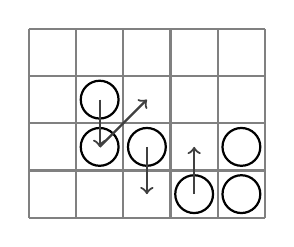
\begin{tikzpicture}[thick, scale=0.6]
    \draw[red,ultra thin,opacity=1] (3,3) node {.};
    \defstuff
    \drawgrid{(5,4)}
    \drawrobots{{(1,2),(1,1),(2,1),(3,0),(4,0),(4,1)}}
    \drawarrows{{{(1,2)/(1,1)},{(1,1)/(2,2)},{(2,1)/(2,0)},{(3,0)/(3,1)}}}
    % \draw[thin] (0,1) -- (3,1) -- (3,4) -- (0,4) -- (0,1);
  \end{tikzpicture}

  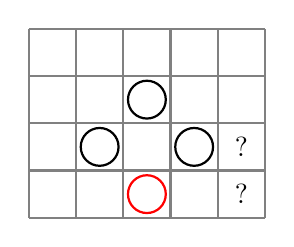
\begin{tikzpicture}[thick, scale=0.6]
    \defstuff
    \drawgrid{(5,4)}
    \drawrobots{{(2,2),(1,1),(3,1)}}
    \drawarrows{{}}
    \draw[red] (2.5,0.5) circle (0.4);
    % \draw[thin] (1,1) -- (4,1) -- (4,4) -- (1,4) -- (1,1);
    \draw (4.5,0.5) node {?};
    \draw (4.5,1.5) node {?};
  \end{tikzpicture}


\end{document}
